
\section{Avaliação Experimental}
	\label{sec:avaliacao-experimental}

%%%%%%%%%% 
% Necessidade de uma referência
%%%%%%%%%%
Para que se possa avaliar um segmentador automático de textos é preciso uma referência, isto é, um texto com os limites entre os segmento conhecidos. Essa referência, deve ser confiável, sendo uma segmentação legítima que é capaz de dividir o texto em porções relativamente independentes, ou seja, uma segmentação ideal.



%%%%%%%%%%
% Formas de conseguir a Segentançaõ de Referência
%%%%%%%%%%
Entre as abordagens mais comuns para se conseguir essas referências, encontramos: 

\begin{itemize}

% Concatenação
\item A concatenação aleatória de documentos distintos, onde o ponto entre o final de um texto e o início do seguinte é um limite entre eles. 

% Segmentação manual
\item A segmentação manual dos documentos, nesse caso, pessoas capacitadas, também chamadas de juízes, ou mesmo o autor do texto, são consultadas e indicam manualmente onde há uma quebra de segmento. 
% Mediador em conversas
\item Em transcrição de conversas faladas em reuniões com múltiplos participantes, um mediador é responsável por encerrar um assunto e iniciar um novo, nesse caso o mediador anota manualmente o tempo onde há uma transição de tópico. 

\end{itemize}

% Não avaliar
Em aplicações onde a segmentação é uma tarefa secundária e quando essas abordagens são custosas ou não se aplicam, é possível, ao invés de avaliar o segmentador, analisar seu impacto na aplicação final.

%%%%%%%%%%
% As 2 principais dificuldades na avaliação
%%%%%%%%%%
De acordo com \cite{Pevzner2002} há duas principais dificuldades na avaliação de segmentadores automáticos. A primeira é conseguir um referência, já que juízes humanos costumam não concordar entre si, sobre onde os limites estão e outras abordagens podem não se aplicar ao contexto. A segunda é que tipos diferentes de erros devem ter pesos diferentes de acordo com a aplicação. Há casos onde certa imprecisão é tolerável e outras, como a segmentação de notícias, onde a precisão é mais importante.


%%%%%%%%%%
% Definição do que é um bom algoritmo de segmentação
%%%%%%%%%%
Para fins de avaliação desse trabalho, um bom método de segmentação é aquele cujo resultado melhor se aproxima do ideal, sem a obrigatoriedade de estar perfeitamente alinhado com tal. Ou seja, visto o contexto das atas de reunião, e a subjetividade da tarefa, não é necessário que os limites entre os segmentos (real e hipótese) sejam idênticos, mas que se assemelhem em localização e quantidade.


%%%%%%%%%%
% Tratamento das atas
%%%%%%%%%%


As próximas subseções mostram o conjunto de atas e a segmentação usada como referência em seguida são apresentadas as métricas de avaliação utilizadas neste trabalho e os testes realizados para avaliar os métodos.


	


\subsection{Medidas de Avaliação}

%%%%%%%%%%
%	Avaliações baseadas em hits 
%%%%%%%%%%

As medidas de avaliação tradicionais, baseiam se na contagem de acertos. No contexto da segmentação de textos um acerto é quando um o limite hipotético coincide com um limite de referência.

Essas medidas de avaliação tentam computar os erros do algoritmo, isto é falsos positivos e falsos negativos, a fim de calcular sua eficiência. 
%
% falso positivo
Um falso positivo é um limite identificado pelo algoritmo que não corresponde a nenhum limite na segmentação de referência. 
%
% falso negativo
Um falso negativo é quando o algoritmo não identifica um limite existente na segmentação de referência.


Nesse sentido, 
%
a precisão, que é a proporção de limites corretamente identificados pelo algoritmo, e 
%
a revocação, que é a proporção de limites verdadeiros que foram identificados pelo algoritmo,
%
trazem alguns problemas na avaliação de segmentadores automáticos.
 	
	
Conforme o algoritmo aponta mais segmentos no texto, este tende a melhorar a revocação e ao mesmo tempo, reduzir a precisão. Esse problema de avaliação pode ser contornado utilizado a medida F-1 que é uma média harmônica entre precisão e revocação onde ambas tem a o mesmo peso. Por por outro lado, tem a desvantagem de ser mais difícil de interpretar. 

As medidas apresentadas acima falham ao não serem sensíveis a \textit{near misses}, ou seja, quando um limite não coincide exatamente com o esperado, mas está próximo a ele~\cite{Kern2009}.

Na Figura~\ref{fig:exemplosegmentacaozoom} é apresentado um exemplo com duas segmentações hipotéticas e uma referência. Na Figura~\ref{fig:exemplosegmentacao}, em ambos os casos não há nenhum verdadeiro positivo, o que implica em zero para os valores de precisão, acurácia, e revocação, embora a segunda hipótese possa ser considerada superior à primeira se levado em conta a proximidade dos limites.



  \begin{figure}[!h]

	\centering
	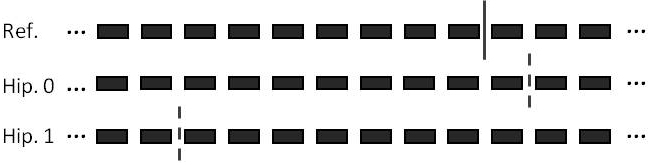
\includegraphics[width=0.47\textwidth]{windiffzoom.jpg}
	\caption{Exemplos de \textit{near missing} e falso positivo puro. Os blocos indicam uma unidade de informação e as linha verticais representam os limites entre segmentos de texto representando um tópico do texto. }
	\label{fig:exemplosegmentacaozoom}

  \end{figure}
  
  \begin{figure}[!h]

	\centering
	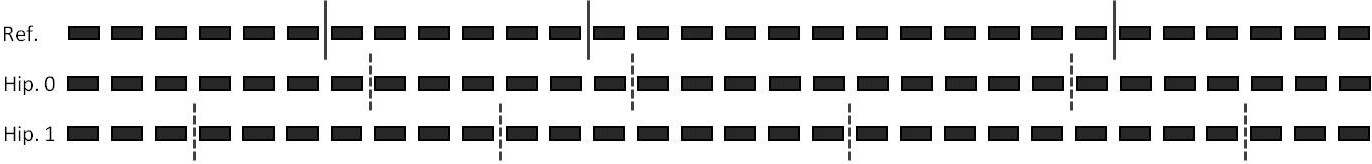
\includegraphics[width=0.47\textwidth]{windiff.jpg}
	\caption{
	Exemplo de duas segmentações hipotéticas em comparação a uma ideal. 
	}
	\label{fig:exemplosegmentacao}

  \end{figure}
  
  
Entre as medidas mais utilizadas para avaliar segmentadores estão:

\begin{enumerate}

	\item P$_k$. A fim de resolver o problema de \textit{near misses}, Beeferman \textit{et. al.}~\cite{Beeferman1999} apresentam uma medida chamada P$_k$ que atribui 
%
valores parciais a \textit{near misses}, 
%
ou seja, limites sempre receberão um peso proporcional à sua proximidade, desde que dentro de um janela de tamanho~$k$.
%
Para isso, esse método move uma janela de tamanho $k$ e a cada posição e verifica se o início e o final da janela estão ou não dentro do mesmo segmento e penaliza o algoritmo em caso de discrepância. Ou seja, dado duas palavras de distancia $k$, uma discrepância é computada quando o algoritmo e a referência não concordam se as palavras estão ou não no mesmo segmento.

O valor de $k$ é calculado como a metade da média dos comprimentos dos segmentos reais. Como resultado, é retornado a contagem de discrepâncias divido pelo quantidade de segmentações analisadas. Esse valor serve como medida de dissimilaridade entre as segmentações e pode ser interpretada como a probabilidade de duas sentenças extraídas aleatoriamente pertencerem ao mesmo segmento.

\item \textit{WindowDiff}. Pevzner~\cite{Pevzner2002} aponta problemas na avaliação mais tradicional, P$_k$~\cite{Beeferman1999}. Eles apontam que esse método penaliza demasiadamente os falsos negativos em relação aos falsos positivos e a \textit{near misses}, além disso, desconsidera o tamanho dos segmentos. Como solução, propõem um método, que traz duas diferenças principais: a dobra da penalidade para os falsos positivos a fim de diminuir o problema da subestimação dessa medida e, diferente de P$_k$, ao mover a janela pelo texto, penaliza-se o algoritmo sempre que o número de limites proposto pelo algoritmo não coincidir com o número de limites esperados para aquela janela de texto. 

Com isso, demonstram em seu trabalho que, em relação a P$_k$, consegue resolver seus principais problemas e mantém sua proposta inicial de sensibilidade a \textit{near misses}, penalizando-os menos que os falsos positivos puros.


\end{enumerate}

\subsection{Configuração experimental}
	\label{subsec:configuracaoexperimental}

%%%%%%%%%%
% Parâmetros
%%%%%%%%%%
As implementações dos algoritmos permitem ao usuário a configuração de seus parâmetros. 
%
O \textit{TextTiling} permite ajustarmos dois parâmetros, sendo, o tamanho da janela (distância entre a primeira e a última sentença) para o qual atribuiu-se os valores 20, 40 e 60. Para o segundo parâmetro, o passo (distância que a janela desliza), atribuiu-se os valores 3, 6, 9 e 12. Gerando ao final 20 modelos.
%

O \textit{C99} permite ajustarmos três parâmetros, sendo, a quantidade segmentos desejados, o qual é calculado como uma proporção dos candidatos a limite. Para isso atribuiu-se as proporções {0,2; 0,4; 0,6; 0,8; 1,0}. O segundo parâmetro, o tamanho do quadro utilizado para gerar a matriz de ranking, atribuiu-se os valores 9 e 11, sendo 11 o valor padrão da apresentado pelo autor. Permite ainda, definirmos se as sentenças serão representados por vetores contendo a frequência ou o peso de cada termo, onde ambas as representações foram utilizadas.
%
 Considerando todos os parâmetros, foram gerados 20 modelos para o algoritmo C99.% By Rafael 


\subsection{Resultados}
	\label{subsec:resultados}

%%%%%%%%%%
% Objetivos
%%%%%%%%%%
A fim de encontrar o melhor método que divida uma ata em segmentos coerentes, realizou-se experimentos com o \textit{TextTiling} e \textit{C99} a fim de encontrar os melhores parâmetros para esses documentos.

%%%%%%%%%%
% Teste de Fiedman e CD
% 1ª Etapa
%%%%%%%%%%
Em seguida aplicou-se o teste de Friedman para saber se há diferenças significativas entre a eficácia dos modelos. O pós-teste de Nemenyi foi aplicado para descobrir quais diferenças são significativas. 
%
Exite diferença quando seus \textit{rankings} médios diferirem em um valor mínimo, chamado de diferença critica (CD). 
%

%%%%%%%%%%
% 
%%%%%%%%%%
Com isso foi possível, pela análise do diagrama de diferença crítica, verificar qual é o melhor modelo para cada medida
% e quão significativamente 
em relação aos demais. 

%%%%%%%%%%
% Dados obtidos com o C99
%%%%%%%%%%
A Tabela~\ref{tab:mediasC99} mostra os dados obtidos com o \textit{C99}, onde \texttt{S} é a proporção de segmentos em relação a quantidade de candidatos, \texttt{M} é o tamanho do quadro utilizado para criar a matriz de \textit{ranking} e \texttt{W} indica se os segmentos são representados por vetores contendo a frequência ou um peso das palavras. 



\begin{table}[!h]
	\centering

	\begin{tabular}{|c|c|c|c|c|}
	
		\hline
		Medida & \texttt{S} & \texttt{M} & \texttt{W} & \textbf{Média}\\		
		\hline

		Acuracy		& 40	& 11 & Sim & 0.6199	\\ \hline	
		F1			& 60	& 9	 & Sim & 0.6167	\\ \hline	
		Precision	& 40	& 11 & Sim & 0.7106	\\ \hline			
		Recall		& 100	& 9	 & Não & 0.8516	\\ \hline		
		Pk			& 40	& 11 & Sim & 0.1163	\\ \hline	
		Windiff		& 40	& 11 & Sim & 0.3800	\\ \hline		

		
	\end{tabular}
	
	\caption{Médias das medidas obtidas com \textit{C99}.}
	\label{tab:mediasC99}
\end{table}


A tabelas~\ref{tab:mediasTextTiling} mostra os dados obtidos com o \textit{TextTiling}, onde \texttt{J} é o tamanho da janela e \texttt{P} é o passo.

\begin{table}[!h]
	\centering

	\begin{tabular}{|c|c|c|c|}
	
		\hline
		Medida & \texttt{J} & \texttt{P} & \textbf{Média}\\		
		\hline

		Acuracy		& 50 & 9 	& 0.5510 \\ \hline	
		F1			& 50 & 3 	& 0.5898 \\ \hline	
		Precision	& 60 & 12 	& 0.5746 \\ \hline			
		Recall		& 50 & 3 	& 0.7717 \\ \hline		
		Pk			& 30 & 9 	& 0.1572 \\ \hline	
		Windiff		& 50 & 9 	& 0.4489 \\ \hline		

		
	\end{tabular}
	
	\caption{Médias das medidas obtidas com o \textit{TextTiling}.}
	\label{tab:mediasTextTiling}
\end{table}


Uma vez sabendo quais valores de parâmetros melhor configuram um algoritmo para uma medida, resta então saber qual dos dois algoritmos é mais eficiente segundo essa medida. Para isso aplicou-se novamente o teste de Friedman com pós-teste de Nemenyi, dessa vez, com os melhores modelos dos dois algoritmos para cada medida. O resultado segue na Tabela~\ref{tab:melhoresmodelos}

\begin{table}[!h]
	\centering
	
	\begin{tabular}{|c|c|c|c|c|}

		\hline
		Medida & Algoritmo & \texttt{S} & \texttt{M} & \texttt{W}\\		
		\hline
		
	
		Acuracy		& C99 & 40 	& 11	& Sim \\ \hline
		Precision	& C99 & 40 	& 11	& Sim \\ \hline
		Pk			& C99 & 40 	& 11	& Sim \\ \hline
		Windiff		& C99 & 40 	& 11	& Sim \\ \hline
		F1			& C99 & 60 	& 9		& Sim \\ \hline
		Recall		& C99 & 100 & 9		& Não \\ \hline
 	
	
	\end{tabular}

	\caption{Melhores modelos para cada medida segundo diagramas de diferença crítica.}
	\label{tab:melhoresmodelos}	
	
\end{table}


Na análise do diagrama de diferença crítica verificou-se que o algoritmo \textit{C99} apresenta melhor eficiência em todas as medidas e os valores das quatro primeiras os valores de \texttt{S}, \texttt{M} e \texttt{W} se repetiram, sugerindo uma configuração otimizada para o problema da segmentação de atas de reunião.




%tópicos retornando segmentos  que retorne segmentos coerentes 




%%%%%%%%%%
% Cálculo das medidas para cada modelo
%%%%%%%%%%

% --> Isso já foi falado no texto
% Pela comparação dos resultados com a segmentação fornecida pelos especialistas, calculou-se para cada modelo as medidas tradicionais acurácia, precisão, revocação, F-medida. 

% Além dessas, computou-se também as métricas mais aplicadas à segmentação textual P$_k$ e \textit{WindowDiff}.


















% ou seja limites não exatos podem ter um peso proporcional à proximidade, desde que estejam dentro da distancia K
%


% Baseando-se em medidas de avaliação tradicionais que utilizam a quantidade de acertos 


%	As medidas de avaliação tradicionalmente utilizadas na área de recuperação de informação como precisão e revocação trazem alguns problemas na avalização de segmentadores automáticos. 
%	
%	se considerarmos 

%	As medidas de avaliação tradicionalmente utilizadas na área de recuperação de informação como  
%
%Precisão é a proporção de limites identificados pelo algoritmo que são verdadeiros
%
%Revocação e a proporção limites verdadeiros que foram identificados pelo algoritmo

%corretamente identificados pelo algorítmo	
	 



%Para quantificar a eficiência dos algoritmos, segue uma revisão das principais métricas aplicáveis.



